\documentclass[12pt,a4paper]{article}

\usepackage[margin=1.2in,headheight=15pt]{geometry}
\usepackage{setspace}
\usepackage[protrusion=true,expansion=false]{microtype}
\usepackage{hyperref}
\usepackage{amsmath,amssymb}
\usepackage[T1]{fontenc}
\usepackage[utf8]{inputenc}
\usepackage{csquotes}
\usepackage{parskip}
\usepackage{titlesec}
\usepackage{fancyhdr}
\usepackage{abstract}
\usepackage{enumitem}
\usepackage{booktabs}
\usepackage[numbers,sort&compress]{natbib}
\usepackage{tikz}
\usepackage{float}

\setcounter{secnumdepth}{3}

\hyphenation{algo-rith-mi-cally neu-ro-psy-cho-ana-ly-sis}

\onehalfspacing

\hypersetup{
    colorlinks=true,
    linkcolor=black,
    urlcolor=black,
    citecolor=black
}

\titleformat{\section}
  {\normalfont\large\bfseries}{\thesection.}{0.75em}{}
\titlespacing*{\section}{0pt}{2.5ex plus 0.5ex minus 0.2ex}{1.2ex plus 0.2ex}

\pagestyle{fancy}
\fancyhf{}
\fancyhead[L]{Flyxion}
\fancyhead[R]{\thepage}
\fancyfoot[C]{\textit{The Hollow Network}}
\renewcommand{\headrulewidth}{0.4pt}

\begin{document}

%% ---------------------------------------------------------------
%%  TITLE PAGE
%% ---------------------------------------------------------------
\begin{titlepage}
\centering
\vspace*{3cm}
{\LARGE\bfseries The Hollow Network\par}
\vspace{1em}
{\large Synthetic Sociality, Metric Misalignment, and the Politics\\[0.3em]
of Legibility in Algorithmically Mediated Environments\par}
\vspace{2em}
{\large Flyxion\par}
\vfill
\end{titlepage}

\setcounter{page}{1}

%% ---------------------------------------------------------------
%%  ABSTRACT
%% ---------------------------------------------------------------
\begin{abstract}
\small
This essay traces the emergence of what it calls \emph{synthetic sociality}---communicative
environments in which the proportion of automated, fabricated, or algorithmically amplified
activity reaches a threshold at which ordinary users can no longer reliably distinguish human
interaction from simulation. Beginning with the phenomenological experience of impersonation,
bot networks, and manufactured content on large social platforms, the essay progressively widens
its explanatory frame. It argues that synthetic sociality is not primarily the product of malicious
actors operating against the interests of platforms, but an emergent property of metric-optimization
systems that treat automated engagement as functionally equivalent to genuine participation. It
further argues that describing platforms as unified rational maximizers misrepresents the
organizational dynamics through which these environments are actually produced---a misrepresentation
compounded, as a structural case study illustrates, by the asymmetry between distributed
operational responsibility and concentrated strategic authority characteristic of founder-led
technology firms. Drawing on historical comparison, the essay considers whether present conditions
represent a novel failure mode or merely the latest iteration of longstanding anxieties about
mediated communication. Three sections extend the argument into the neuropsychoanalytic register,
drawing on Karl Friston's Free Energy Principle \citep{friston2010} and Lacanian theory
\citep{lacan2006,dallaglio2024} to explain why synthetic environments are so effective at
capturing and organizing human attention. A further section draws a structural analogy from
recent work in flow-based generative models \citep{gloy2025} to characterize the information
architecture underlying synthetic social environments. The essay concludes that the central
problem is not the existence of synthetic activity but its opacity and involuntary character,
and that the appropriate design response centers on informational legibility, provenance, and
the transformation of synthetic interaction from a hidden structural condition into a transparent
and consensual one.
\end{abstract}

\vspace{1em}
\noindent\textbf{Keywords:} synthetic sociality, algorithmic platforms, engagement metrics,
platform governance, online fraud, predictive coding, Free Energy Principle, jouissance,
neuropsychoanalysis, information flow

\newpage

%% ---------------------------------------------------------------
%%  SECTION 1
%% ---------------------------------------------------------------
\section{The Perceptual Contradiction}

There is a peculiar dissonance at the center of contemporary social media. The largest platforms
are also, by their own account, among the most sophisticated artificial intelligence laboratories
in existence. Their research divisions publish widely in machine learning, their infrastructure
processes billions of interactions daily, and their public communications consistently frame
artificial intelligence as a transformative project: a technology that will improve content
moderation, personalize discovery, and deepen the quality of human connection across networks of
unprecedented scale \citep{zuboff2019,wu2016}.

Yet the everyday experience of using these platforms increasingly consists of something quite
different. An ordinary user logging into a major social network today is likely to encounter
impersonation accounts cloning the profile photographs and names of people they know, coordinated
bot networks producing and amplifying content at velocities no human community could sustain, and
entire pages or channels composed of synthetic or recycled video assembled by automated pipelines
optimized not for meaning but for engagement signals. The friend request from a duplicate account,
the adoption listing that collects a deposit and then vanishes, the comment thread where suspiciously
similar accounts converge on an identical talking point---these are not marginal experiences but
routine features of the social environment these platforms have built \citep{gillespie2018}.

I use the term \emph{synthetic sociality} to describe communicative environments in which
automated, fabricated, or algorithmically amplified actors constitute a sufficiently large
proportion of visible activity that users can no longer reliably distinguish genuine social
interaction from simulation. The concept is not evaluative in the first instance: it describes
a structural condition of the environment rather than a moral failing of any particular actor.
Its explanatory purpose is to name what users already experience---that interacting on large
social platforms increasingly resembles navigating a space populated by simulations---and to
make that experience available for systematic analysis.

This creates an initial puzzle. If a company invests billions in frontier AI research, why does
its platform feel crowded with crude identity scams? If recommendation algorithms operate at a
level of sophistication that can model individual attention patterns across hundreds of millions
of users, why cannot the same organization reliably detect when an account has cloned a photograph
from another profile and is soliciting money from that person's contacts?

The easy answer---that these are simply different technical problems, and that malicious actors
are an inevitable presence in any large open system---is not wrong, but it is insufficient. It
treats the distribution of engineering effort as though it were a natural phenomenon, a consequence
of difficulty rather than of institutional choice. The harder question is why certain capabilities
receive resources and others do not, and what those priorities reveal about the actual objectives
these organizations are designed to pursue \citep{tufekci2015}.

%% ---------------------------------------------------------------
%%  SECTION 2
%% ---------------------------------------------------------------
\section{The Infrastructure Alibi}

The initial explanation most commonly offered for the proliferation of synthetic activity on social
platforms is structural. Large-scale automation infrastructure, the argument goes, is inherently
dual-use. The same pipelines that allow legitimate applications---content recommendation,
advertising targeting, automated customer service---necessarily lower the barrier for actors
pursuing illegitimate ends. A platform that makes it easy to distribute video at scale makes it
equally easy for a reel farm to flood the recommendation system with manufactured content. A
network that allows rapid account creation enables both authentic participation and mass-produced
impersonation.

This explanation is accurate as far as it goes. The technical infrastructure of large platforms
does not distinguish, at a fundamental level, between human activity and automated mimicry of
human activity. Both produce signals---clicks, watch time, shares, follow actions---that the
system is built to process and respond to. There is no architectural feature of a recommendation
pipeline that inherently privileges genuine human intention over automated approximation of it
\citep{pariser2011,vosoughi2018}.

But the structural explanation carries an implicit exculpatory logic. By framing synthetic
activity as an unfortunate side effect of general-purpose infrastructure, it positions the platform
as a neutral party whose tools have been turned against it by external malicious actors. The
platform, in this framing, is struggling with a problem that has been imposed on it from outside---
adversaries exploiting infrastructure that was designed for better purposes.

This framing has rhetorical utility. It allows companies to speak simultaneously about their
commitment to safety and their investment in AI without confronting the possibility that these
two commitments might be in tension. It also determines which interventions appear natural: if
the problem is external adversaries exploiting legitimate infrastructure, the solution is better
detection and enforcement---a security problem, technical in character, requiring engineering
resources but not organizational reflection \citep{gillespie2018}.

What the framing does not address is the prior question of why the infrastructure was built
without authenticity requirements in the first place, and why it has remained without them as
the scale and sophistication of synthetic activity has become increasingly legible. The gap
between organizational rhetoric and platform experience is not incidental; it is, as Zuboff
observes of surveillance capitalism more broadly, a structural feature of systems whose economic
logic is oriented around the extraction and monetization of behavioral data rather than around
the quality of communicative experience \citep{zuboff2019}.

%% ---------------------------------------------------------------
%%  SECTION 3
%% ---------------------------------------------------------------
\section{Metric Indifference and Its Beneficiaries}

A stronger interpretation of the phenomenon requires attending more carefully to what social
platforms actually optimize and for whom. The dominant metric across large consumer platforms
is some variant of engagement: click-through rates, watch time, shares, daily active users,
time on platform. These indicators began as proxies for something that seemed genuinely
meaningful---evidence that people were finding value in the network, that content was
resonating, that the platform was doing its job of connecting people with things they wanted
to see \citep{wu2016}.

The moment these proxies became the primary optimization target of both internal systems and
external reporting, however, they acquired a different character. Goodhart's Law---the principle
that when a measure becomes a target, it ceases to be a reliable measure of what it originally
represented---describes the resulting dynamic with precision \citep{strathern1997}. Once
engagement metrics entered the objective functions of recommendation algorithms, quarterly
reports, and engineering performance reviews, the system's behavior reoriented around the
production of those metrics rather than around whatever underlying quality they were originally
meant to indicate.

We can formalize the dynamic briefly. Let $E(A)$ denote the engagement produced by activity
$A$ in the platform environment. The optimization problem the system actually solves is:

\begin{equation}
\max_{A} \; E(A) \quad \text{subject to operational constraints}
\label{eq:engmax}
\end{equation}

The critical observation is that if authenticity---the property that $A$ represents genuine
human expression or communication---does not appear in $E$, then it is invisible to the
objective function. An automated account that watches a video long enough to register a
completion event, triggers a recommendation to another account, and generates a share action
produces exactly the same signal as a human performing identical interactions. From the
perspective of the optimization system, these are equivalent \citep{tufekci2015}.

This equivalence is not merely a technical artifact; it has economic consequences. Advertising
markets are primarily concerned with impressions and interaction signals. An automated impression
that generates a measurable interaction is, from the standpoint of the advertising transaction,
indistinguishable from a human one---provided the fraud does not reach a scale that advertisers
can detect and penalize. At moderate levels, automated activity can actually stabilize platform
metrics, filling engagement gaps when human participation fluctuates and providing consistent
throughput for recommendation pipelines \citep{bakshy2015}.

The implication is uncomfortable but analytically unavoidable. Platforms do not merely tolerate
synthetic activity because it is technically difficult to eliminate. They operate in conditions
where synthetic activity produces measurable signals that their business model treats as
positive---at least below whatever threshold would attract regulatory scrutiny or advertiser
defection. The relationship between the platform and the synthetic activity is therefore not
cleanly adversarial. It is, at minimum, one of mutual indifference, and in some respects one
of mutual benefit \citep{zuboff2019}.

This does not require deliberate deception. It can arise from something more mundane: a system
designed to maximize measurable signals, encountering a class of activity that produces those
signals, and failing to develop the capacity to distinguish it from the activity the signals
were meant to represent. The absence of malice does not, however, diminish the structural
condition. An optimization system that is indifferent to authenticity will produce environments
in which authenticity is not protected, regardless of what the organization professes in its
public communications \citep{gillespie2018,noble2018}.

%% ---------------------------------------------------------------
%%  SECTION 4
%% ---------------------------------------------------------------
\section{Against the Unified Maximizer}

There is a danger in the analysis developed so far, which is that it generates too clean a
picture. Writing the system as~(\ref{eq:engmax}) implies the existence of a coherent agent
with a well-defined objective function. Large technology companies are not like this. They are
bureaucratic organizations of tens or hundreds of thousands of people, distributed across
divisions that have different mandates, different time horizons, and sometimes directly
competing incentives \citep{gillespie2018}.

An engineering team building recommendation infrastructure is rewarded for model performance
on engagement metrics. A trust-and-safety team is rewarded for the volume of policy violations
detected and removed. A product team is rewarded for user growth and retention numbers. A policy
team responds to regulatory pressure and manages relationships with governments and civil society
organizations. Each of these teams optimizes for a locally defined objective. The interaction
of these locally optimized systems produces the overall behavior of the organization---but that
behavior does not have the coherence one would expect if a single agent were solving a single
problem \citep{tufekci2015}.

This matters because it changes the diagnosis of why synthetic activity persists. The answer
may not be that the company has made a strategic decision to tolerate bots because they inflate
metrics. It may be something more dispersed: that the team with the mandate to address
coordinated inauthentic behavior has insufficient resources relative to the teams building the
infrastructure that enables it; that detection of sophisticated synthetic networks requires
capabilities that cross organizational boundaries and therefore fall into gaps between divisions;
that the metrics by which senior leadership evaluates platform health do not include indicators
of synthetic activity that would make its prevalence visible; or simply that the problem is
technically difficult and the organization's attention is directed elsewhere by immediate
competitive pressures.

These organizational dynamics are not exculpatory---they explain rather than excuse---but they
do have implications for how change might occur. An organization that has made a strategic choice
to prioritize engagement over authenticity might be moved by changes in regulation, advertising
market pressure, or public discourse to shift that choice. An organization whose behavior toward
synthetic activity emerges from distributed organizational dysfunction requires different
interventions: changes to internal measurement systems, resource allocation, and promotion
criteria that bring the stated commitment to authenticity into alignment with the incentive
structures that actually govern day-to-day decisions \citep{noble2018,zuboff2019}.

The institutional explanation also draws attention to a pattern that appears across many
organizations managing complex infrastructures at scale: the gap between what an organization
publicly commits to and what its internal incentive architecture actually rewards tends to be
visible precisely in the areas where commitment would be costly. Eliminating synthetic activity
aggressively might shrink reported user bases, reduce engagement metrics, and create friction
in content distribution pipelines---all of which would appear as negative signals in the
reporting structures by which large platforms are evaluated. This is not a conspiracy; it is
the ordinary operation of institutional incentives \citep{strathern1997}, and it is why
commitments to authenticity that are not embedded in measurable internal targets tend to
remain symbolic.

%% ---------------------------------------------------------------
%%  SECTION 5  [NEW: Distributed Responsibility]
%% ---------------------------------------------------------------
\section{Distributed Responsibility and Concentrated Power}

A structural pattern in the governance of large technology firms compounds the organizational
dynamics described above. Contemporary platform companies have increasingly adopted what might
be called a portfolio model of technical leadership: distributing operational responsibility
across multiple semi-autonomous groups while preserving concentrated strategic authority at
the top of the organizational hierarchy \citep{gillespie2018}.

This arrangement is typically justified on grounds of organizational agility. By distributing
development work across several teams, a company can pursue parallel approaches, reduce
dependence on any single technical leader, and avoid the bottlenecks associated with hierarchical
decision-making. Parallel experimentation is a rational strategy for managing uncertainty in
domains---such as frontier AI research---where the technical landscape is genuinely unpredictable
and failure is both common and informative.

The governance implication of this structure, however, is less straightforward than the
managerial rationale suggests. Operational responsibility is distributed widely across
specialized groups, but ultimate strategic authority remains tightly concentrated. In founder-led
technology firms, this concentration is frequently reinforced through voting share arrangements
and board control that make the formal authority of the founder structurally immune to the
diffusion of operational risk that other parts of the organization are subject to
\citep{zuboff2019}.

The result is a characteristic institutional geometry. When initiatives succeed, success accrues
upward to visionary leadership. When they fail, responsibility is distributed laterally across
a network of teams whose mandates overlap and whose accountability relationships are genuinely
complex. This asymmetry between the distribution of operational risk and the concentration of
strategic power is not unique to technology firms, but it is particularly consequential in
organizations that govern communicative infrastructures of societal scale.

The asymmetry has a direct bearing on the persistence of synthetic sociality. When no single
organizational actor bears clear accountability for the aggregate informational environment the
platform produces, the cumulative effect of many locally optimized decisions---each of which
may appear defensible in isolation---can produce systemic conditions for which no one is
institutionally responsible. The impersonation network that exploits the easy account-creation
pipeline, the coordinated bot farm that games the engagement algorithm, and the scam page that
exploits the absence of provenance verification are each addressable by specific teams. The
systemic condition that makes all three simultaneously viable and persistent belongs to no team's
mandate.

This observation reinforces the argument against treating the platform as a unified maximizer
while complicating the available remedies. Changing the objective function of a coherent
organization is challenging but conceptually tractable. Restructuring accountability relationships
in an organization whose behavior emerges from many semi-independent teams, each optimizing
locally, and whose ultimate authority is structurally insulated from operational consequences,
requires intervention at a different level---one that goes beyond internal reform toward
regulatory frameworks capable of imposing accountability at the point where strategic authority
and operational impact actually converge \citep{tufekci2015,noble2018}.

%% ---------------------------------------------------------------
%%  SECTION 6
%% ---------------------------------------------------------------
\section{The Externalization of Cost}

The analysis of platform incentives acquires a sharper moral character when considered from
the perspective of the people who bear the consequences of synthetic activity. The asymmetry
between those who create fraud and those who experience it is not accidental. It is structured
by the same institutional indifference that allows synthetic activity to persist within the
optimization environment \citep{noble2018}.

Consider the range of fraud enabled by the conditions described above. Impersonation accounts
clone a person's photograph, name, and fragments of their public posts to create convincing
duplicates, which are then used to solicit money from the original person's contacts or to
distribute fraudulent links to their audience. Fake rehoming pages for animals accept deposits
from people seeking to adopt pets and then disappear, with the operator moving to a new page
or a different regional community group. Rental scams collect deposits on apartments that do
not exist or are not available for rent, exploiting the trust that platform community membership
implies. Investment fraud accounts build apparent legitimacy through stolen identity signals
before promoting schemes to extract money from followers.

These are not sophisticated attacks. They exploit elementary features of platform design: the
ease of account creation without identity verification, the absence of meaningful history or
provenance signals for new accounts, the capacity to operate across jurisdictions and communities
without accountability to any of them, and the availability of algorithmic amplification that
places new content in front of large audiences before any reputation has been established
\citep{gillespie2018,tufekci2015}.

The cost of this fraud is borne almost entirely by individuals. A person who has lost a deposit
to a rental scam must determine, individually, whether and how to pursue recovery---a process
that is time-consuming, often fruitless, and emotionally taxing. A person whose identity has been
impersonated must navigate reporting systems that may respond slowly or inconsistently, while
their contacts continue to receive fraudulent messages from the duplicate account. The platform
removes an account if and when it violates policy; the network behind it persists and generates
new accounts.

This pattern reflects a broader principle about the distribution of costs in systems with weak
accountability mechanisms. In offline contexts, fraud encounters friction: social networks impose
reputational costs on deception that is discovered, legal systems create deterrence, and the
geographic and social proximity of fraudulent activity to its victims creates pressure toward
accountability. None of these friction mechanisms operate effectively in large digital environments
with low barriers to account creation and identity change \citep{boyd2014}.

The jarring quality of this situation is the contrast between the organizational resources
directed toward capability development and the relative thinness of basic protective
infrastructure. It is not primarily a technical problem that a platform investing at scale in AI
systems cannot build reliable identity verification, enforce against repeat fraudulent operators,
or surface provenance information for accounts and content. It is an institutional problem: the
investments that would address these failures do not register as improvements in the metrics by
which these organizations are governed and evaluated \citep{wu2016,zuboff2019}.

One might observe that analogous dynamics existed long before digital platforms. Gossip and
rumor in small communities could damage reputations without recourse; fraudulent operators in
physical marketplaces found ways to exploit trust and disappear. A single piece of misinformation
circulating through a workplace or neighborhood could undo years of carefully built trust, and
the individual targeted had no institutional recourse. The platforms are not inventors of social
deception. What they have done is remove the friction that historically constrained its scale
\citep{boyd2014}. In a small community, the same social network that transmitted rumor also
limited its reach and eventually created accountability. On a platform serving hundreds of
millions of users across thousands of communities, an operator can exploit each community in
sequence, moving faster than any single community can respond, with no mechanism for coordination
among victims that would produce collective pressure on the institution hosting the activity.

%% ---------------------------------------------------------------
%%  SECTION 7
%% ---------------------------------------------------------------
\section{The Historical Mirror}

Before concluding that contemporary platforms represent a wholly unprecedented failure, it is
worth submitting the diagnosis to historical comparison. Anxieties about the authenticity of
mediated communication have accompanied nearly every significant communication technology.
The introduction of print raised concerns that the proliferation of texts would overwhelm the
reader's capacity for critical evaluation. Broadcasting was accused of manufacturing false
consensus, homogenizing culture, and replacing genuine political participation with the
appearance of it---a critique developed at length in Debord's analysis of the society of the
spectacle \citep{debord1967} and in Postman's account of how television restructured public
discourse around entertainment rather than argument \citep{postman1985}. Early internet forums
generated extensive discussion about the unreliability of anonymous communication and the
impossibility of verifying the identity or sincerity of interlocutors \citep{boyd2014}.

In each case, critics worried that technological mediation would displace authentic human contact
with a cheaper substitute---that the medium would produce environments populated by
representations and performances rather than genuine persons. And in each case, the prediction
was partially vindicated and partially refuted: new media did introduce new forms of manipulation
and inauthenticity, and human communities found ways to develop new norms, literacies, and
institutions that allowed meaningful interaction to persist alongside the degraded forms.

The question for contemporary platforms is whether they represent merely the latest iteration of
this recurrent anxiety or whether they introduce failure modes that are qualitatively different
from what preceded them. There are grounds for arguing that some features of the current
situation are genuinely novel. Earlier mass media manipulated at scale but lacked personalization:
a propaganda campaign addressed the same message to a mass audience. Contemporary platforms
combine algorithmic personalization, granular data about social relationships, and the capacity
to generate synthetic identities that can operate inside individual social networks rather than
broadcasting to an undifferentiated public \citep{vosoughi2018,bakshy2015}.

An impersonation account that clones a specific person's identity and operates within that
person's actual social graph---sending messages to their actual friends and colleagues---is
categorically different from a mass-media propaganda campaign. It exploits the intimacy of
personal relationship rather than the diffuse attention of a public audience. It is harder to
detect because it does not feel like mass communication; it feels like a message from someone
the recipient knows. And it can be generated at scale with minimal cost, targeting thousands of
individual social contexts simultaneously in ways that no earlier technology permitted
\citep{vosoughi2018}.

This qualitative distinction matters because it determines what forms of literacy and institutional
response are appropriate. Teaching people to be skeptical of anonymous strangers on early internet
forums was a reasonable response to that environment. Teaching people to suspect messages from
accounts that appear to be their friends and family members, while not technically unreasonable
as advice, points toward the collapse of a social environment rather than its maintenance
\citep{tufekci2015}.

%% ---------------------------------------------------------------
%%  SECTION 8
%% ---------------------------------------------------------------
\section{The Complexity of Desire}

Any account of what has gone wrong with social platforms must grapple honestly with the complexity
of what users actually want. The analysis so far has implicitly treated the preference for authentic
human interaction as given, and the proliferation of synthetic activity as a deviation from that
preference that users would eliminate if given the choice. This is not obviously correct
\citep{boyd2014}.

Many people engage willingly and knowingly with automated or semi-automated communicative actors.
Parasocial relationships with content creators who interact with audiences through algorithmically
optimized posting schedules, brand accounts that communicate through automated responses, and
entertainment streams produced by coordinated content teams are all widely chosen forms of digital
interaction \citep{wu2016}. They are often attractive precisely because they require no
reciprocity: the engagement is one-directional, the social obligation minimal, and the experience
of connection available without the cost of genuine relationship.

This complexity does not undermine the critique of involuntary synthetic activity, but it refines
it. The problem users experience is not simply the existence of automated actors in their social
environments. It is the specific character of that automation: deceptive, opaque, and
non-consensual. The impersonation account is objectionable not because it is automated but
because it claims to be something it is not, exploiting the trust that authentic identity implies.
The coordinated bot network is problematic not because it involves multiple accounts but because
it simulates the appearance of independent consensus that does not exist. The rental scam is
harmful not because it uses digital tools but because it exploits the informational asymmetry
those tools create \citep{gillespie2018,noble2018}.

The distinction between consensual and non-consensual synthetic interaction is therefore crucial.
A user who knowingly follows an automated entertainment account is making a choice about how to
allocate their attention. A user who receives a message from what appears to be their colleague
and is in fact an impersonation account has had that choice made for them---and made against
their interests. The design challenge is to make the boundary between these two conditions
visible rather than to eliminate one of them.

%% ---------------------------------------------------------------
%%  SECTION 9
%% ---------------------------------------------------------------
\section{The Predictive Subject}

The institutional critique developed so far explains why synthetic social environments arise.
To understand why they are so effective, however, we must also consider the structure of the
human cognitive apparatus that interacts with these environments. The analysis of platform
incentives is incomplete without a corresponding account of why manufactured signals are so
difficult to resist, and why the same person who is intellectually aware that engagement-bait
is manufactured continues to respond to it.

Contemporary computational neuroscience increasingly describes the brain not as a passive
recorder of sensory data but as a \emph{predictive system} \citep{friston2010,solms2021}.
Rather than waiting to receive information, the brain continuously generates hypotheses about
the causes of sensory input and updates these hypotheses when predictions fail. Karl Friston's
Free Energy Principle (FEP) formalizes this process: biological systems must minimize long-run
informational surprise in order to remain within the viable states characteristic of their kind
\citep{friston2010,friston2013}.%
\footnote{Friston, ``The Free-Energy Principle: A Unified Brain Theory?''
\emph{Nature Reviews Neuroscience} 11 (2010): 127--138.}

In the FEP framework, let $s$ denote sensory input and $z$ the hidden states of the world
that generate it. The brain maintains an approximate posterior $q(z)$ over these hidden states.
Variational free energy $F$ is defined as:

\begin{equation}
F = D_{\mathrm{KL}}\!\bigl(q(z)\,\|\,p(z|s)\bigr) - \ln p(s)
\label{eq:fep}
\end{equation}

where $D_{\mathrm{KL}}$ is the Kullback--Leibler divergence between the brain's approximate
beliefs and the true posterior, and $-\ln p(s)$ is the log-surprise of sensory observations.
Because the brain cannot access $p(z|s)$ directly, minimizing $F$ serves as a tractable proxy
for minimizing surprise itself \citep{friston2010}.

This minimization proceeds through two complementary strategies. The first, \emph{perception},
involves updating internal beliefs $q(z)$ to better explain incoming sensory signals. The
second, \emph{action}, involves changing the environment so that sensory signals conform to
predictions. The brain is therefore not a passive observer but an active inference engine:
it continuously generates hypotheses and acts to confirm them. Within this architecture,
emotionally salient signals are assigned \emph{precision}---a weighting that determines which
prediction errors receive attention and drive behavioral reorganization. High-precision errors
propagate upward through the predictive hierarchy and compel the system to revise its models
or act; low-precision errors are treated as noise \citep{friston2013,solms2021}.

The psychoanalytic tradition anticipated aspects of this architecture long before predictive
coding models existed. Lacan's formulation that the unconscious is structured like a language
\citep{lacan2006} describes a system organized around chains of signifiers that attempt to
stabilize experience by providing expectations against which incoming signals are measured.
These symbolic chains function analogously to the priors of predictive coding: they organize
perception by supplying expectations against which incoming signals are measured. The
contemporary neuropsychoanalytic synthesis of Friston and Lacan, developed at length in
Dall'Aglio \citep{dallaglio2024} and in the clinical work of Solms \citep{solms2021}, treats
the FEP as providing the neurobiological substrate through which Lacanian structural claims
can be understood empirically.

The subject that emerges from this architecture is not a unified rational agent. It is a
predictive system divided between competing sources of expectation, affect, and symbolic meaning.
The Lacanian notation for this condition is the \emph{barred subject} ($\$$), a formal marker
indicating that the subject is constitutively split between what it consciously knows and the
forces that organize its desire from positions it cannot fully occupy \citep{lacan2006,dallaglio2024}.
This divided predictive subject is particularly vulnerable in environments where informational
signals are intentionally manipulated. When synthetic actors imitate social cues---identity
markers, emotional signals, apparent consensus---they exploit precisely the mechanisms through
which predictive brains construct their models of reality.

Crucially, the brain does not sit behind its Markov blanket as an impartial observer. It
\emph{self-evidences}: it acts upon the world to produce sensory data that confirms its
generative models \citep{friston2013}. This means that a platform environment designed to
elicit high-precision emotional responses does not merely attract attention passively---it
actively recruits the brain's own inference machinery into the service of engagement
maximization.

%% ---------------------------------------------------------------
%%  SECTION 10
%% ---------------------------------------------------------------
\section{Jouissance and Surplus Prediction Error}

While predictive models emphasize the brain's tendency to minimize error, psychoanalysis insists
that human subjects often repeat experiences that generate distress rather than reducing it.
This paradox was articulated by Freud as the repetition compulsion \citep{freud1920} and later
formalized by Lacan through the concept of \emph{jouissance}---a paradoxical form of enjoyment
that persists beyond the pleasure principle. Jouissance is not simply pleasure but a surplus of
excitation that the subject repeatedly encounters even when, and sometimes especially when, it
produces suffering \citep{lacan2006,dallaglio2024}.

Within predictive neuroscience, this phenomenon can be understood as a form of \emph{surplus
prediction error}. The brain's seven basic emotional systems, identified in Panksepp's affective
neuroscience \citep{panksepp1998}, function as what the FEP framework calls \emph{hyperpriors}:
innate, high-precision predictions that must be confirmed by experience. These systems---among
them SEEKING, FEAR, PANIC, RAGE, and CARE---register deviations from socio-emotional homeostasis
as \emph{felt uncertainty}. Unlike cortical prediction errors, which can be resolved by updating
beliefs, these subcortical errors demand action: they cannot be ``thought away''
\citep{panksepp1998,solms2021}.

When a particular emotional uncertainty acquires extremely high precision weighting---when the
system assigns it disproportionate salience---the entire predictive hierarchy reorganizes around
resolving it, even when repeated attempts fail. In Lacanian notation, the signifier that carries
this excessive weight is the \emph{master signifier} $S_1$: a term that does not convey semantic
content but resonates with the weight of jouissance, organizing the subject's life around a
kernel of unresolved tension \citep{lacan2006}. The Lacanian \emph{objet~$a$}---the object-cause
of desire---is not a thing but a formal gap within the predictive model itself: the residual
uncertainty that cannot be eliminated and that ensures the SEEKING system never fully shuts down
\citep{dallaglio2024,panksepp1998}.

This structural feature of human cognition has direct implications for the analysis of synthetic
sociality. Content optimized for engagement does not arbitrarily capture attention; it does so
by targeting precisely those emotional frequencies that carry the highest natural precision.
Outrage, fear, the threat of social exclusion, the promise of hidden knowledge---these are
high-precision prediction errors that the brain is constitutively unable to ignore
\citep{vosoughi2018,friston2013}. The recommendation algorithm that learns to surface such
content is not deceiving users in the straightforward sense; it is exploiting the brain's own
error-prioritization mechanism, causing the brain to repeatedly return to stimuli that produce
the neurological signature of importance without delivering resolution.

The result is recognizable as what the Lacanian clinic calls jouissance in its mortifying form:
an enjoyment that immobilizes rather than satisfies, that organizes behavior around a recurring
gap rather than moving toward closure \citep{dallaglio2024}. The user scrolling through an
algorithmically curated feed of outrage, anxiety, and manufactured social consensus is not simply
distracted. They are caught in a loop that exploits the predictive brain's most primitive
response to unresolved uncertainty---they keep looking because the signal design ensures the
prediction error never settles \citep{friston2010,vosoughi2018}.

There is also a specifically institutional dimension here. The brain's tendency to automatize
responses to familiar patterns---to reduce the metabolic cost of conscious processing by
routinizing interaction \citep{solms2021}---creates an additional vulnerability. Prematurely
automatized predictions, formed in conditions of comparative helplessness, persist as rigid
behavioral templates even when they fail to satisfy adult needs \citep{dallaglio2024}. Platform
environments that continuously reinforce habitual engagement patterns exploit this tendency
toward automatization, gradually moving interaction from reflective engagement toward compulsive
behavioral loops.

%% ---------------------------------------------------------------
%%  SECTION 11
%% ---------------------------------------------------------------
\section{Clinical Insight: Precision, Manipulation, and the Analytic Position}

Psychoanalytic practice provides an unexpected perspective on these dynamics, instructive
precisely because it has developed, over decades of clinical refinement, techniques for
intervening in the precision-weighting of signifiers---that is, for disrupting the rigid
assignments of salience that organize symptomatic repetition \citep{lacan2006,dallaglio2024}.

Within the Lacanian clinic, the analyst does not attempt to eliminate the subject's symptoms
by replacing them with better beliefs, as cognitive-behavioral approaches largely do. Instead,
analytic technique seeks to intervene in the structure of the subject's predictive hierarchy
by modulating the precision of specific signifiers. Two classical techniques are illuminating.

\emph{Punctuation} refers to the act of emphasizing particular terms within the patient's
speech, effectively shifting their symbolic weight. By marking a signifier that the patient
treats as transparent---one they speak through rather than about---the analyst introduces a
precision perturbation that forces the predictive system to attend to what it had been silently
organizing \citep{lacan2006}. \emph{Scansion}, the practice of ending a session at a point of
unresolved tension, prevents the patient's narrative from achieving the closure that would allow
the brain's secondary revision to discharge the prediction error and return the system to
automatized prediction \citep{dallaglio2024}. By holding the uncertainty open, the analyst
exploits the same principle that platform designers exploit: sustained high-precision prediction
error demands engagement.

The critical difference is ethical. In the clinical context, these interventions are deliberate,
transparent in their therapeutic purpose, and directed toward the patient's own singular
relationship to their desire---toward what Lacan called the \emph{ethics of desire} \citep{lacan2006},
a non-normative position that does not prescribe what the subject should want but creates
conditions in which they can encounter what they actually do want. The goal is not to produce a
subject who conforms to a statistical norm of psychological health but to enable the subject to
develop what Dall'Aglio describes as a way to manage the structural tension of the drive---to
find a singular relationship to the irreducible surplus of jouissance rather than being
organized by it unconsciously \citep{dallaglio2024}.

In algorithmically mediated environments, analogous mechanisms operate without transparency or
consent, and with the opposite therapeutic orientation \citep{zuboff2019}. Recommendation systems
continuously amplify the signals that produce highest engagement---which, as argued above,
correlates strongly with emotionally salient uncertainty \citep{vosoughi2018}. The system
effectively performs a large-scale experiment in precision manipulation across the entire
population of users, systematically increasing the salience of specific prediction errors within
the collective attention economy. The subject thus produced is not one who has developed a
reflective relationship to their desire but one whose desire has been captured, organized, and
stabilized around the platform's own optimization target \citep{zuboff2019,dallaglio2024}.

The neuropsychoanalytic perspective therefore converges with the institutional analysis from a
different direction. Platform environments do not merely expose users to synthetic content; they
actively reorganize the predictive architectures of their users over time. A person who has
spent years having their precision-weighting manipulated by algorithmically optimized content is
not simply better informed about the existence of synthetic sociality. They are a different kind
of predictive subject---one whose habitual salience assignments have been trained by an environment
indifferent to their flourishing \citep{solms2021,dallaglio2024}.

%% ---------------------------------------------------------------
%%  SECTION 12 — The Political Economy of Jouissance
%% ---------------------------------------------------------------
\section{The Political Economy of Jouissance}

The preceding discussion suggests that psychological symptoms may be understood as locally
stable solutions to the problem of managing uncertainty. In digital environments governed by
algorithmic recommendation systems, however, these dynamics become embedded within a broader
economic structure. The resulting system can be interpreted as a political economy organized
around the extraction and amplification of affective uncertainty.

In Dall'Aglio's synthesis, the Lacanian concept of \emph{jouissance} is interpreted through
the predictive brain framework as the subjective experience of persistent prediction error
\citep{dallaglio2024}. Rather than representing a simple failure of cognitive processing,
jouissance corresponds to the affective intensity produced when uncertainty cannot be fully
resolved by the subject's generative model. From a psychoanalytic perspective, the subject is
not merely disturbed by this condition but becomes attached to it: jouissance represents the
paradoxical enjoyment of the gap between expectation and experience, and the subject repeatedly
encounters the same unresolved tension because it organizes desire itself \citep{lacan2006}.

Digital platforms introduce a structural transformation of this dynamic. Recommendation
algorithms operate by identifying signals that reliably produce engagement. In practice, these
signals are often associated with affectively charged content---material that provokes surprise,
anxiety, outrage, curiosity, or unresolved tension. Within the predictive processing framework,
such stimuli correspond to large prediction errors: content that confirms existing expectations
produces minimal informational change, whereas content that disrupts expectations produces
strong prediction-error signals that capture attention \citep{friston2010}.

This asymmetry produces a structural alignment between platform incentives and the affective
mechanics of the predictive brain. Systems optimized for engagement will naturally converge on
stimuli that produce high-magnitude prediction errors. In doing so, they amplify the very
conditions that generate jouissance. The result is an informational economy that systematically
harvests unresolved uncertainty. Users remain within cycles of affective stimulation because
the platform continuously supplies signals that maintain prediction errors without allowing them
to resolve into stable knowledge or meaningful social closure \citep{vosoughi2018,zuboff2019}.

This dynamic helps explain the persistent emotional volatility characteristic of contemporary
online discourse. The system does not simply distribute information; it organizes attention
around the repeated activation of affective prediction errors. In this sense, the hollow
network described throughout this essay can be interpreted as a system that produces the
affective signals of social interaction without the stabilizing processes through which social
meaning is normally constructed. The user experiences continual engagement, yet the underlying
uncertainty remains unresolved.

Within the RSVP formalism, prediction error corresponds to gradients in the entropy field
$\mathcal{S}(x,t)$: $\epsilon \sim \nabla\mathcal{S}$. Platform amplification mechanisms
therefore act as external forces that continually reinforce regions of high informational
gradient in the plenum. The resulting attractor states correspond to persistent affective loops
in which uncertainty is repeatedly stimulated but rarely resolved. Under these conditions,
digital platforms become infrastructures that convert human attention into a resource by
stabilizing the subjective experience of irreducible uncertainty.

%% ---------------------------------------------------------------
%%  SECTION 13 — Bracketing, Sheaves, and the Geometry of Jouissance
%% ---------------------------------------------------------------
\section{Bracketing as Region Formation in the Spherepop Sheaf}

The political economy of jouissance outlined above raises the question of how meaning is
locally constructed and why its global closure so frequently fails. A precise answer requires
attending to the cognitive operations through which agents bound their interpretive fields.
The discussion that follows unifies three analytical languages---phenomenological bracketing,
predictive-processing inference, and Spherepop region formation---into a single formal
structure, and then extends that structure into the geometry of sheaf theory to show that
jouissance is not merely an affective condition but a topological one.

\subsection*{Bracketing as Conditional Inference}

Cognitive systems cannot evaluate all possible hypotheses simultaneously. Phenomenology
describes the restriction of interpretive attention through the concept of \emph{bracketing}
(\emph{epoch\'{e}}): the suspension of portions of the world in order to examine a particular
structure of experience. Mathematically, this operation corresponds to conditioning inference
over a restricted domain.

Let the full informational environment be represented as a space of possible events
$\Omega = \{e_1, e_2, \dots, e_n\}$. A generative model maintains a probability distribution
$p(e)$ over this space. Bracketing corresponds to restricting inference to a subset
$B \subset \Omega$, after which inference is performed over the conditional distribution
$p(e \mid B)$.

\subsection*{Spherepop Regions}

In the Spherepop framework, meaning is constructed through irreversible event histories.
Events are represented as nodes in a directed causal structure $G = (E, R)$, where $E$ is
the set of events and $R$ is the set of causal relations. A \emph{Spherepop region} is a
connected subgraph $\mathcal{R}_i = (E_i, R_i)$ with $E_i \subset E$. Interpretation occurs
not over the full graph but within these bounded regions.

The structural equivalence between phenomenological bracketing and Spherepop regions can then
be stated directly. Bracketing selects $B \subset \Omega$ while Spherepop defines
$\mathcal{R}_i \subset E$: both operations restrict inference to a bounded informational
structure. Constructing a Spherepop region performs the same logical operation as
phenomenological bracketing; the difference lies only in implementation. Bracketing occurs
at the level of subjective attention, whereas Spherepop performs the operation computationally
by partitioning event histories into coherent regions.

Within the RSVP plenum, prediction error becomes region-specific: $\epsilon_i \sim \nabla\mathcal{S}|_{\mathcal{R}_i}$.
Each region thus functions as a localized domain of uncertainty management. Regions with
persistent entropy gradients correspond to stable affective attractors---precisely the
structures associated with jouissance. Recommendation systems alter the informational
landscape by preferentially amplifying regions with large entropy gradients, so that the
digital environment gradually reorganizes itself around attractor regions of unresolved
affective prediction error \citep{zuboff2019,vosoughi2018}.

\subsection*{Spherepop Regions as Sheaves Over Event Graphs}

The equivalence between bracketing and Spherepop regions can be made more precise using the
mathematical language of sheaf theory \citep{zuboff2019}. Sheaf theory describes how locally
defined structures can be consistently glued together into global objects, and has been
applied to distributed systems and multi-agent information processing. It is particularly
well suited to environments in which different observers possess partial and locally
consistent views of a shared informational structure.

Let the event graph $G = (E, R)$ be treated as a topological space by defining a collection
of open sets $\mathcal{U} = \{U_i\}$ with $U_i \subseteq E$. Each open set represents a
region of causally proximate events. A sheaf $\mathcal{F}$ assigns informational content to
each open set: for each region $U$, $\mathcal{F}(U)$ is the set of interpretations---beliefs,
semantic structures, predictive models---constructed by agents within that region. For
$V \subseteq U$, there exists a restriction map $\rho_{U,V} : \mathcal{F}(U) \to \mathcal{F}(V)$
describing how interpretations over a larger region restrict to a smaller one.

The central property of a sheaf is that locally consistent interpretations can be glued into
a global interpretation when compatibility conditions are satisfied. If a collection of regions
$U_i$ covers a larger region $U = \bigcup_i U_i$, and if interpretations $s_i \in \mathcal{F}(U_i)$
agree on their overlaps---$\rho_{U_i, U_i \cap U_j}(s_i) = \rho_{U_j, U_i \cap U_j}(s_j)$
for all $i,j$---then there exists a unique global section $s \in \mathcal{F}(U)$ gluing the
local interpretations together. This mathematical condition corresponds directly to the process
through which agents construct shared meaning from locally consistent perspectives.

\begin{figure}[H]
\centering
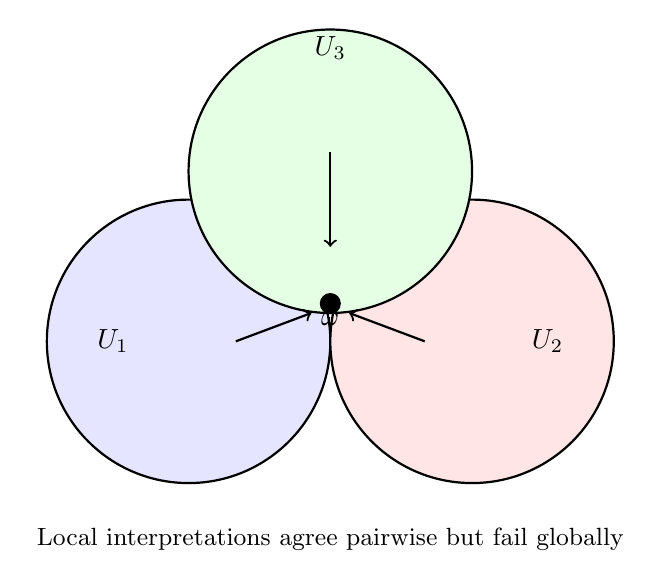
\begin{tikzpicture}[scale=1.2]
\draw[thick, fill=blue!10] (-1.5,0) circle (1.5);
\draw[thick, fill=red!10] (1.5,0) circle (1.5);
\draw[thick, fill=green!10] (0,1.8) circle (1.5);
\node at (-2.3,0) {$U_1$};
\node at (2.3,0) {$U_2$};
\node at (0,3.1) {$U_3$};
\filldraw[black] (0,0.4) circle (3pt);
\node[below] at (0,0.4) {$\omega$};
\draw[->, thick] (-1,0) -- (-0.2,0.3);
\draw[->, thick] (1,0) -- (0.2,0.3);
\draw[->, thick] (0,2) -- (0,1);
\node at (0,-2.1) {\small Local interpretations agree pairwise but fail globally};
\end{tikzpicture}
\caption{Sheaf obstruction representing jouissance: local interpretive regions $U_i$ admit
consistent sections, but no global section exists due to the obstruction $\omega$.}
\label{fig:sheaf-obstruction}
\end{figure}

\subsection*{The Geometry of Jouissance}

Sheaf theory also allows for situations in which no global section exists: when local
interpretations are internally consistent but incompatible when extended across the entire
system, the structure possesses only partial sections. This property mirrors the psychoanalytic
insight that meaning is often structured around irreducible gaps or contradictions, and in
predictive-processing terms these gaps correspond to persistent prediction errors
\citep{dallaglio2024}.

In Lacanian terms, jouissance names the persistence of an excess that cannot be fully
symbolized \citep{lacan2006}. In the Spherepop-sheaf formalism, these two descriptions
converge: jouissance can be modeled as a topological obstruction preventing the gluing of
locally coherent interpretations into a single global section.

Let $s_i \in \mathcal{F}(U_i)$ be a local section---internally coherent and even pairwise
compatible with others---yet failing to extend to a global section $s \in \mathcal{F}(U)$
satisfying $\rho_{U,U_i}(s) = s_i$ for all $i$. In cohomological language, jouissance appears
when there is a nontrivial obstruction class in the first \v{C}ech cohomology group:

\[
[\omega] \in \check{H}^{1}(G,\mathcal{F}), \qquad [\omega] \neq 0.
\]

Under this interpretation, jouissance corresponds not to the local sections themselves but to
the persistent obstruction they circle around. The Lacanian \emph{objet~$a$} becomes
mathematically legible as the minimal residual inconsistency that keeps the interpretive
system in motion: not a positive object but the structured remainder of failed global closure
\citep{dallaglio2024,lacan2006}.

This formalism clarifies why jouissance is so readily captured by digital platforms.
Recommendation systems need not understand the full semantic content of a user's interpretive
field; they need only identify regions in which unresolved incompatibilities generate
persistent attention and affective return. Writing the amplification weight $A(U_i)$ assigned
to each region, the economically valuable regions are those for which local interpretive
density is high while global closure fails:

\[
A(U_i) \propto \|\epsilon_i\| \cdot \chi\!\left([\omega]_{U_i} \neq 0\right),
\]

where $\chi$ is an indicator function marking the presence of a nontrivial obstruction. The
platform preferentially amplifies not resolved meanings but unresolved interpretive knots.
This is why the political economy of engagement aligns so closely with the dynamics of
jouissance: the most profitable regions are precisely those where local significance is high
and global integration is impossible.

Within the RSVP formalism, this obstruction corresponds to a persistent entropy singularity:

\[
\oint_{\partial U_i} \nabla\mathcal{S} \cdot d\ell \neq 0,
\]

expressing that the system is not merely noisy but topologically knotted around a persistent
inconsistency. Spherepop's role now becomes more precise: if current platforms profit by
circulating users around unresolved obstructions, Spherepop seeks to re-embed those
obstructions within durable event histories whose provenance can be tracked, contested, and
recursively refined. Its aim is not to abolish inconsistency---which would be both impossible
and undesirable---but to transform blind repetition into legible structure. An obstruction
that is merely exploited traps the subject in an affective loop; an obstruction that becomes
available for shared interpretation becomes the site of collective waymaking.

\begin{figure}[H]
\centering
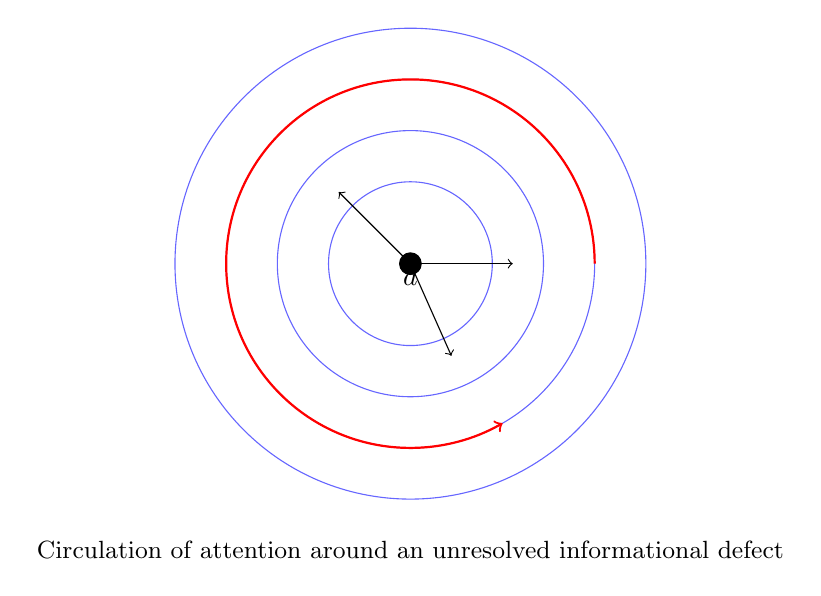
\begin{tikzpicture}[scale=1.3]
\foreach \r in {0.8,1.3,1.8,2.3} {
  \draw[blue!60] (0,0) circle (\r);
}
\filldraw[black] (0,0) circle (3pt);
\node[below] at (0,0) {$a$};
\draw[->, thick, red] (1.8,0) arc (0:300:1.8);
\draw[->] (0,0) -- (1,0);
\draw[->] (0,0) -- (-0.7,0.7);
\draw[->] (0,0) -- (0.4,-0.9);
\node at (0,-2.8) {\small Circulation of attention around an unresolved informational defect};
\end{tikzpicture}
\caption{Jouissance as circulation around a persistent entropy defect in the RSVP plenum. The
central point $a$ is the \emph{objet~$a$}---not a positive object but the structured remainder
of failed global closure. Attention repeatedly orbits without achieving resolution.}
\label{fig:jouissance-defect}
\end{figure}

%% ---------------------------------------------------------------
%%  SECTION 14 — Dynamic Bracketing and Constellations
%% ---------------------------------------------------------------
\section{Dynamic Bracketing and Constellations of Interpretation}

The previous section described Spherepop regions as subsets of the event graph arising through
acts of phenomenological bracketing. This description risks suggesting that regions are static
partitions of the informational environment. In practice, interpretive regions are continuously
reorganized by the activity of agents navigating the informational field. The boundaries of
attention shift as new events occur, as prior interpretations are revised, and as participants
renegotiate the meaning of earlier interactions.

The language of \emph{waymaking}---the ongoing movement through which agents maintain
coherence within a changing environment---describes this process philosophically. From this
perspective, bracketing is not a single operation but a continuous process of selecting and
reselecting interpretive boundaries. The subject constructs temporary regions of relevance in
order to orient itself within a larger field of possibilities.

The metaphor of the constellation is useful here. A constellation does not exist as a fixed
object in the sky; it emerges from the act of connecting particular stars into meaningful
patterns, and different observers may draw different constellations from the same stellar
background. Similarly, interpretive regions arise from the activity of agents who connect
events into coherent structures: these structures are neither purely subjective nor fully
determined by the underlying environment but are negotiated patterns formed within the
informational field.

Spherepop formalizes this process by representing interpretive regions as dynamically evolving
covers of the event manifold. Let the informational environment be represented as an event
manifold $M$ whose points correspond to events and whose local structure is defined by causal
relations between them. Agents navigating this manifold construct temporary regions of
interpretation $U_i \subset M$. At any moment, these regions form an open cover
$\mathcal{U} = \{U_1, U_2, \dots, U_k\}$ such that $M = \bigcup_{i=1}^k U_i$.

As new events occur, the cover changes: regions expand, contract, or recombine. This
time-dependent cover $\mathcal{U}(t) = \{U_1(t), U_2(t), \dots\}$ evolves according to

\[
\frac{dU_i}{dt} = f\!\left(U_i,\, \nabla\mathcal{S},\, E\right),
\]

where $E$ denotes new events entering the manifold and $\nabla\mathcal{S}$ represents entropy
gradients within the RSVP plenum. Waymaking is precisely this continuous reconfiguration of
the cover as agents adjust their interpretive boundaries in response to prediction error.

A \emph{constellation} can be defined as a connected substructure $C \subset U_i$ in which
events form a coherent trajectory. These constellations function as semantic anchors within
the informational field, guiding future interpretation and influencing how new events are
bracketed. Large prediction errors force agents to restructure the cover: an event $e$ either
expands an existing region, $U_i(t+\Delta t) = U_i(t) \cup \{e\}$, or, if it destabilizes
prior interpretation, triggers contraction, $U_i(t+\Delta t) = U_i(t) \setminus V$. In this
sense, waymaking is the continuous re-bracketing of the event manifold in response to the
entropy structure of the RSVP plenum.

\begin{figure}[H]
\centering
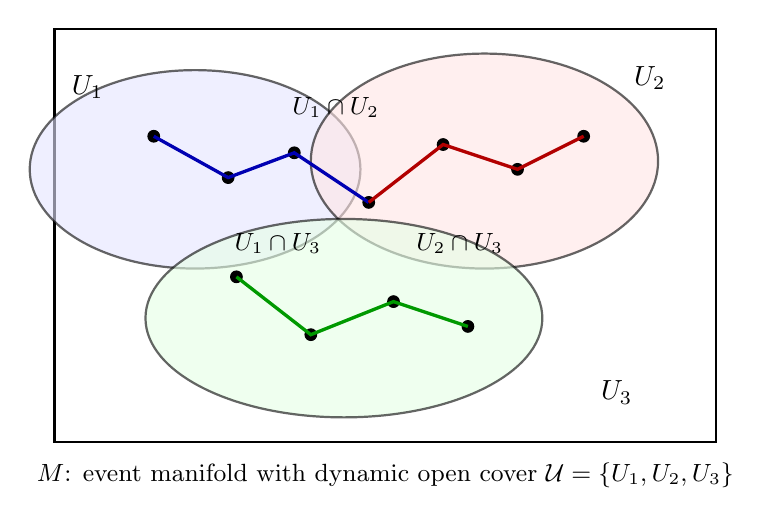
\begin{tikzpicture}[scale=1.05]
\draw[thick] (-4,-2.5) rectangle (4,2.5);
\draw[thick, fill=blue!10, opacity=0.6] (-2.3,0.8) ellipse (2.0 and 1.2);
\draw[thick, fill=red!10, opacity=0.6] (1.2,0.9) ellipse (2.1 and 1.3);
\draw[thick, fill=green!10, opacity=0.6] (-0.5,-1.0) ellipse (2.4 and 1.2);
\node at (-3.6,1.8) {$U_1$};
\node at (3.2,1.9) {$U_2$};
\node at (2.8,-1.9) {$U_3$};
\filldraw (-2.8,1.2) circle (2pt);
\filldraw (-1.9,0.7) circle (2pt);
\filldraw (-1.1,1.0) circle (2pt);
\filldraw (-0.2,0.4) circle (2pt);
\filldraw (0.7,1.1) circle (2pt);
\filldraw (1.6,0.8) circle (2pt);
\filldraw (2.4,1.2) circle (2pt);
\filldraw (-1.8,-0.5) circle (2pt);
\filldraw (-0.9,-1.2) circle (2pt);
\filldraw (0.1,-0.8) circle (2pt);
\filldraw (1.0,-1.1) circle (2pt);
\draw[very thick, blue!70!black] (-2.8,1.2) -- (-1.9,0.7) -- (-1.1,1.0) -- (-0.2,0.4);
\draw[very thick, red!70!black] (-0.2,0.4) -- (0.7,1.1) -- (1.6,0.8) -- (2.4,1.2);
\draw[very thick, green!60!black] (-1.8,-0.5) -- (-0.9,-1.2) -- (0.1,-0.8) -- (1.0,-1.1);
\node at (-0.6,1.55) {\small $U_1 \cap U_2$};
\node at (-1.3,-0.1) {\small $U_1 \cap U_3$};
\node at (0.9,-0.1) {\small $U_2 \cap U_3$};
\node at (0,-2.9) {\small $M$: event manifold with dynamic open cover $\mathcal{U}=\{U_1,U_2,U_3\}$};
\end{tikzpicture}
\caption{Spherepop regions as a dynamic open cover of the event manifold. Constellations are
connected interpretive paths within and across local regions; overlaps are sites of shared
meaning where gluing conditions must be negotiated.}
\label{fig:event-manifold}
\end{figure}

Digital platforms intervene in this process by algorithmically reshaping the informational
environment. Recommendation systems selectively amplify certain events, altering the entropy
landscape of the RSVP plenum and biasing the formation of interpretive regions. The
constellations that emerge are therefore not purely products of collective interpretation but
are partially engineered by the platform's optimization dynamics. The open cover of the event
manifold becomes skewed toward regions that maximize engagement rather than regions that
support stable knowledge formation. The hollow network is, in these terms, a distortion of the
interpretive cover of the informational manifold. A Spherepop-enabled infrastructure proposes
an alternative in which event histories remain legible, and reversible structures of
interpretation can emerge through collective waymaking rather than algorithmic manipulation.

%% ---------------------------------------------------------------
%%  SECTION 15 — Waymaking as Path-Integration in the RSVP Plenum
%% ---------------------------------------------------------------
\section{Waymaking as Path-Integration in the RSVP Plenum}

The formal model developed in the preceding sections describes the informational environment
as a scalar-vector-entropy field in which events produce perturbations and agents attempt to
stabilize their generative models in response to those perturbations. While this formalism
captures the structural dynamics of the informational plenum, it does not yet account for the
lived activity through which agents navigate that field.

The concept of \emph{waymaking} provides a crucial bridge between the geometry of the RSVP
plenum and the agency of the subject. Where the RSVP framework describes the field of
informational potential, waymaking describes the process by which an agent moves through that
field while maintaining its own structural coherence---a continuous process of path-integration
within the informational landscape. The agent maintains a trajectory through the plenum while
adjusting its internal model in response to entropy gradients and unexpected perturbations.
This transforms the informational field from a passive background into a navigational
environment: the subject does not merely receive signals but actively participates in shaping
its trajectory through a landscape of possibilities.

Within the predictive processing framework, this activity corresponds to the ongoing attempt
of the generative model to reduce prediction error while preserving the structural integrity
of the organism \citep{friston2010}. The subject continually adjusts its expectations, actions,
and attention in order to maintain a viable relationship with the surrounding environment.
In the language of care ethics and embodied cognition, this movement can be interpreted as a
form of \emph{constitutive care}: the organism sustains itself through a precarious balancing
act between order and uncertainty. Too much rigidity results in brittle models that cannot
adapt to change, while excessive uncertainty leads to disorientation and loss of form.
Waymaking involves the maintenance of a dynamic equilibrium within the informational field.

Within the RSVP framework, waymaking can be expressed as the movement of an agent through the
scalar-vector-entropy field. Let the informational state of the plenum be
$\Psi(x,t) = (\Phi, \mathbf{v}, \mathcal{S})$. An agent's trajectory through this field is
represented as a path $\gamma(t) \subset \Psi$. The dynamics of navigation are influenced by
entropy gradients $\nabla\mathcal{S}(x,t)$, and waymaking corresponds to the continuous
adjustment of the trajectory in response to these gradients:

\[
\frac{d\gamma}{dt} = -\nabla\mathcal{S} + \eta,
\]

where $\eta$ represents exploratory variation generated by the agent. The maintenance of
structural coherence requires that the trajectory remain within viable informational bounds
$\|\gamma(t)\| < \kappa$, where $\kappa$ represents the stability threshold of the agent's
generative model.

The hollow network disrupts this process by replacing the agent's navigational activity with
algorithmically generated trajectories. Recommendation systems predict and precompute the
informational paths that users are likely to follow, presenting stimuli designed to maximize
engagement rather than to support genuine exploratory navigation. As a result, the subject's
role shifts from active navigator to passive consumer of algorithmically generated pathways.
Instead of engaging in waymaking, the user is effectively \emph{way-made} by the platform's
optimization process---a shift with significant implications for cognitive development and
social agency, since the struggle of navigation is removed and the subject loses the
opportunity to engage in the interpretive labor through which knowledge and meaning are
constructed.

%% ---------------------------------------------------------------
%%  SECTION 16 — The Erosion of Productive Friction
%% ---------------------------------------------------------------
\section{The Erosion of Productive Friction}

The concept of waymaking introduced in the previous section highlights the importance of
navigational agency in cognitive and social systems. Agents sustain themselves not by
eliminating uncertainty altogether but by continuously negotiating it. The process of
navigation requires a balance between stability and exploration, between prediction and
surprise.

Work in embodied cognition emphasizes that this tension is not a defect of the cognitive
system but its primary generative force. Genuine learning occurs when agents encounter
situations that challenge their existing models yet remain interpretable through interaction
and reflection. This tension can be described as \emph{productive friction}: the encounter
with uncertainty that stimulates interpretive effort and adaptive reorganization.

Modern digital platforms are typically designed according to a different principle. User
experience design prioritizes the elimination of friction in order to create seamless
interaction flows. Recommendation systems attempt to predict user preferences with increasing
precision, presenting stimuli that minimize the cognitive effort required to select or
interpret content. While such optimization may appear beneficial in the short term, it has
profound consequences for the dynamics of waymaking. When the informational environment is
continuously pre-structured by predictive algorithms, the subject is relieved of the
responsibility to navigate uncertainty independently.

In effect, the platform substitutes its own objective function for the exploratory activity of
the agent. Instead of negotiating multiple possible trajectories through the informational
landscape, the user encounters a curated sequence of stimuli optimized for engagement. This
shift alters the relationship between prediction error and learning: under normal conditions,
prediction error stimulates interpretive activity that gradually reduces uncertainty; in
algorithmically optimized environments, however, prediction error is artificially modulated
in order to sustain attention without facilitating genuine understanding. The result is an
informational ecology characterized by oscillations between novelty and familiarity that
maintain engagement while limiting the depth of cognitive restructuring. The subject receives
continuous stimulation yet rarely encounters the productive difficulty required for meaningful
conceptual change.

From the perspective of the RSVP framework, the elimination of friction corresponds to the
suppression of exploratory variance in the agent's trajectory. When algorithms continuously
adjust the environment to match predicted preferences, the entropy gradients encountered by
the subject are carefully controlled, and the agent is guided along paths that maximize
engagement while minimizing navigational effort. Over time this process can lead to cognitive
atrophy: the capacities required for autonomous waymaking---interpretation, deliberation, and
communicative assessment---are progressively displaced by passive consumption of
algorithmically generated trajectories.

In this sense the hollow network is not merely hollow because it contains synthetic signals,
but because it systematically removes the productive friction through which meaning and
understanding are normally constructed. The informational environment becomes smooth and
frictionless, yet this very smoothness undermines the generative processes through which
cognition develops.

Formally, let exploratory variance in navigation be expressed as a stochastic component
$\eta(t)$ such that $\frac{d\gamma}{dt} = -\nabla\mathcal{S} + \eta$. Algorithmic optimization
suppresses this exploratory variance by introducing an external guiding function $A(\gamma,t)$
which biases the trajectory toward predicted engagement states:

\[
\frac{d\gamma}{dt} = -\nabla\mathcal{S} + A(\gamma,t).
\]

When $A$ dominates the dynamics, exploratory variance approaches zero, $\eta \to 0$, and the
system loses its capacity for genuine waymaking. Navigation is replaced by externally guided
trajectories optimized for engagement rather than understanding.

%% ---------------------------------------------------------------
%%  SECTION 17 — Sympoiesis and the Infrastructure of Co-Creation
%% ---------------------------------------------------------------
\section{Sympoiesis and the Infrastructure of Co-Creation}

The previous sections argued that the hollow network arises when the process of waymaking is
replaced by algorithmically precomputed trajectories and when productive friction is
systematically removed from the informational environment. If cognition depends upon
negotiating uncertainty, then infrastructures that eliminate this negotiation undermine the
conditions under which meaning can emerge. A constructive response therefore requires more
than simply reducing synthetic activity or improving moderation systems; it requires
rethinking the architecture of the informational environment itself.

One conceptual framework that helps articulate such an alternative is the notion of
\emph{sympoiesis}. Originally developed in biological and ecological contexts, sympoiesis
describes systems that are collectively produced rather than centrally controlled \citep{boyd2014}.
In a sympoietic system, structure emerges through the interactions of multiple agents rather
than through the directives of a single organizing authority. This contrasts sharply with the
\emph{autopoietic} infrastructure of contemporary digital platforms, which operate as
centrally optimized systems whose primary objective functions are determined by internal
metrics such as engagement, advertising revenue, and growth. Users interact with one another
only through the mediation of algorithms whose primary role is to guide attention according
to the platform's optimization strategy.

A sympoietic informational infrastructure would operate according to a different principle.
Instead of precomputing the trajectories of attention, it would provide a shared environment
in which agents collectively construct the informational landscape. Within such an environment,
meaning emerges through interaction, interpretation, and negotiation among participants rather
than through algorithmic orchestration.

The Spherepop framework can be understood as an attempt to provide the technical infrastructure
required for such a system. The key principle is the irreversibility of event histories: each
interaction produces an event that is permanently recorded as part of a shared informational
trajectory, transforming the informational environment from a collection of ephemeral signals
into a structured history of interactions. Where contemporary platforms primarily manage streams
of content, Spherepop manages trajectories of events, allowing participants to reconstruct the
provenance of information and to evaluate its meaning within the context of prior interactions.

From the perspective of the RSVP plenum, irreversible event histories introduce a stabilizing
structure into the informational field. Events induce perturbations $e_i \to \delta\Psi_i(x,t)$,
and the accumulation of events generates a stratified structure of historical layers:

\[
\Psi(x,t) = \Psi_0 + \sum_i \delta\Psi_i.
\]

Agents navigating this environment therefore encounter not merely isolated signals but
historically grounded informational structures. This historical grounding enables collective
waymaking: participants can orient themselves relative to shared trajectories of interaction
rather than relying solely on algorithmically generated recommendations. In this sense,
Spherepop provides the structural conditions necessary for sympoiesis. Meaning arises through
the ongoing coordination of multiple agents within a shared informational history, and the
hollow network fails precisely because it suppresses this historical grounding.

The transition from a hollow network to a sympoietic infrastructure can be described as the
transformation of informational flows into structured event trajectories. Let
$E = \{e_1, e_2, \dots, e_n\}$ represent the sequence of events produced by interacting
agents. The informational structure of the system can then be expressed as a directed event
graph $G = (E, R)$ where $R$ represents causal relations between events. Collective waymaking
corresponds to the emergence of coherent paths within this graph:

\[
\Gamma = \{e_{i_1} \to e_{i_2} \to \cdots\}.
\]

These paths represent shared trajectories of interpretation and interaction. In a sympoietic
informational infrastructure, the stability of these paths determines the coherence of the
social environment. Meaning therefore emerges not from the optimization of engagement metrics
but from the sustained coordination of event trajectories across the informational plenum.

%% ---------------------------------------------------------------
%%  SECTION 18  [formerly 12: HollowFlow / information architecture]
%% ---------------------------------------------------------------
\section{Hollow Flows: The Architecture of Constrained Propagation}

The dynamics described in previous sections---engagement optimization, coordinated synthetic
activity, and the exploitation of predictive cognitive architectures---are further illuminated
by a structural analogy from an adjacent technical domain. Recent work in flow-based generative
modeling has addressed a computational problem whose formal structure bears a suggestive
resemblance to the informational architecture of large social platforms.

In systems designed to evaluate sample likelihoods over high-dimensional probabilistic graphs,
a fundamental difficulty arises as dependency structures become dense: evaluating likelihoods
requires integrating across an exponentially growing set of computational paths, a cost that
rapidly becomes prohibitive. The approach developed in \citet{gloy2025} addresses this by
enforcing a \emph{hollow} internal structure---specifically, a block-diagonal Jacobian
constraint combined with non-backtracking message passing---that restricts the pathways through
which information can propagate within the model. By preventing recursive loops of mutual
influence, the architecture ensures that signals move through well-defined forward channels,
making likelihood evaluation tractable even at large scale.

The relevance of this structure to the argument of this essay is not technical but conceptual.
Social platforms of the scale under discussion here appear, from the user's perspective, as
dense communicative networks in which information circulates freely among millions of
participants. In practice, however, the pathways through which content actually reaches attention
are highly constrained. Algorithmic ranking systems, recommendation pipelines, and engagement
optimization mechanisms define narrow channels through which signals are amplified or
attenuated. The appearance of a rich conversational network conceals an informational
architecture that is, in the sense made precise by \citet{gloy2025}, effectively hollow: one
whose visible density masks the structural thinness of the channels through which meaningful
circulation actually occurs.

This hollowness has two consequences that are directly relevant to the persistence of synthetic
sociality. First, because the channels through which content propagates are defined by engagement
optimization rather than by epistemic criteria, synthetic signals---bot posts, reel farms,
coordinated inauthentic behavior---compete on exactly equal terms with authentic ones. Both enter
the same constrained amplification channels; both are evaluated by the same engagement metric.
The architecture provides no internal mechanism for distinguishing a signal that is widely
amplified because it is genuinely resonant from one that is widely amplified because an automated
network has been designed to trigger the channel's amplification criteria.

Second, and more subtly, the constrained channel structure means that the apparent diversity of
information circulating on a large platform substantially overstates the actual diversity of the
informational environment users encounter. Content that successfully enters the amplification
channels recirculates widely; content that does not essentially disappears from the social
surface of the network. The result is an environment that feels saturated with information while
being, in terms of the pathways through which attention actually flows, quite narrow---one in
which synthetic actors who have learned to game the amplification criteria can achieve visibility
disproportionate to their authenticity or epistemic quality \citep{vosoughi2018,tufekci2015}.

The title of this essay is, in part, an allusion to this structural condition. A hollow network
is not an empty one; it may be densely populated with signals and interactions. What is hollow
is the relationship between the apparent structure of the network---its visible sociality---and
the actual architecture of information flow that underlies it. That discrepancy between surface
and structure is the formal condition that makes synthetic sociality possible at scale.

%% ---------------------------------------------------------------
%%  SECTION 13
%% ---------------------------------------------------------------
\section{Opacity and the Predictive Trap}

The reframing from inauthenticity to opacity---developed in the institutional analysis and now
deepened by both the neuropsychoanalytic account and the structural analysis of information
flow---allows a more precise diagnosis of what has gone wrong. The question is not whether
social platforms should contain automated actors, synthetic content, or algorithmically mediated
interaction; in some sense they cannot avoid containing all of these. The question is whether
the nature of the actors and the status of the content are \emph{legible} to users, and whether
users have the cognitive and informational resources to calibrate their predictive models
accordingly \citep{gillespie2018}.

Opacity operates at several levels. At the level of identity, accounts that represent automated
systems or organized promotional campaigns are often indistinguishable from accounts representing
individual humans, because the platform provides insufficient provenance information to make the
distinction. At the level of content, media that has been synthetically generated or repurposed
from other contexts frequently circulates without indicators of origin \citep{vosoughi2018}.
At the level of behavior, coordinated networks of accounts that simulate independent opinion
formation are designed to be invisible as networks---their coordination is the feature that makes
them effective, and the platform's infrastructure does not surface that coordination to users
encountering their output \citep{tufekci2015}.

From the predictive brain's perspective, opacity is not a neutral condition. The brain calibrates
precision according to its models of source reliability \citep{friston2013}. A message that
appears to come from a trusted contact carries higher precision than one from an unknown account,
precisely because the generative model of ``trusted contact'' includes strong priors about the
signal's likely accuracy and relevance. Opacity exploits this calibration: by simulating the
surface features of trusted sources, synthetic actors inherit precision that they have not earned.
The prediction error they introduce therefore bypasses the skeptical filters that the brain would
apply to signals from unknown sources \citep{dallaglio2024,solms2021}.

The consequences of opacity for trust are significant. When users cannot determine whether the
account sending them a message represents a person they know, an automated system, or an
organized fraud network, the epistemic status of every interaction is degraded. The rational
response is generalized suspicion---a posture that damages genuine communication alongside
fraudulent simulation \citep{boyd2014}. The cost of this degradation falls unevenly:
sophisticated users with the time and resources to investigate suspicious activity bear it
differently than users who lack those capacities \citep{noble2018}.

The burden of verification has been externalized to individual users in a system that provides
them with insufficient tools to perform it. This is the institutional failure at the center of
the problem. A communication infrastructure operating at the scale of the major social platforms
is not simply a marketplace of ideas in which users are responsible for their own epistemic
hygiene. It is an environment whose design choices determine what information is available to
whom, and those choices currently distribute informational disadvantage downward---toward users
who are least equipped to compensate for it \citep{noble2018,zuboff2019}.

%% ---------------------------------------------------------------
%%  SECTION 14
%% ---------------------------------------------------------------
\section{Legibility as Infrastructure}

The appropriate response to the opacity problem is not to attempt the elimination of synthetic
activity from social environments---an impossible goal, and arguably not a desirable one given
that many forms of automation serve genuine user interests. The appropriate response is to treat
informational legibility as infrastructure: a basic feature of the communicative environment
that the platform is responsible for providing, in the same way that electrical infrastructure
is responsible for grounding, or financial infrastructure is responsible for disclosure
\citep{gillespie2018,zuboff2019}.

Concretely, this means several things. Identity provenance should be surfaced rather than
obscured: accounts representing individuals, organizations, automated systems, or coordinated
campaigns should carry indicators that allow users to understand what kind of communicative
actor they are engaging with. This does not require the elimination of pseudonymity, which serves
legitimate purposes; it requires distinguishing between human-controlled pseudonymous accounts
and non-human or coordinated actors. Content origin should be similarly legible: media that has
been synthetically generated, repurposed from other contexts, or distributed by automated
pipelines should carry provenance indicators that are visible to the user encountering it
\citep{tufekci2015}.

Enforcement against repeat fraudulent operators should treat the underlying network, not merely
the individual account, as the unit of accountability. A scammer who creates a new page after
having a previous one removed has not been meaningfully deterred; the infrastructure has simply
absorbed the cost of their continuation. Effective enforcement requires coordinating across
account histories, behavioral patterns, and network connections in ways that make the operational
friction of fraud substantially higher than the current environment imposes \citep{gillespie2018}.

User controls should allow people to choose the degree of synthetic interaction they wish to
engage with. A user who prefers to see only content from verified human accounts should have
mechanisms to accomplish this. A user who is comfortable engaging with automated entertainment
accounts should be able to do so knowingly. The goal is not to homogenize the social environment
but to transform the current condition---in which synthetic interaction is an ambient, hidden
structural feature---into one in which it is a transparent option \citep{boyd2014}.

These interventions require institutional commitment that goes beyond stated values. They require
that the measurement systems, promotion criteria, and resource allocation decisions inside large
platforms treat legibility as a performance indicator in the same way that engagement is currently
a performance indicator \citep{strathern1997}. They require that the costs of fraud---which are
currently externalized to individual users---be recognized as costs attributable to platform
design, and that accountability for those costs be located at the institutional level where the
relevant design choices are made \citep{noble2018,zuboff2019}.

The neuropsychoanalytic argument adds a further dimension to this demand \citep{dallaglio2024,friston2010}.
If it is true that sustained exposure to opacity and precision manipulation gradually reorganizes
the predictive architectures of users, then legibility is not only a matter of fairness in
individual transactions. It is a matter of the cognitive conditions required for genuine agency.
A user whose salience-weighting has been trained by years of algorithmically optimized
manipulation is not simply uninformed about synthetic content; their capacity for the kind of
reflective self-determination that meaningful choice requires has been partially colonized
\citep{zuboff2019,dallaglio2024}. Legibility, in this deeper sense, is a precondition for the
kind of subject who is capable of exercising the consent that the design proposal assumes.

%% ---------------------------------------------------------------
%%  SECTION 15
%% ---------------------------------------------------------------
\section{Conclusion: The Redesign of Trust}

The experience of contemporary social media that motivates this essay---fake accounts, synthetic
reels, adoption scams, impersonation fraud---is best understood not as the failure of technology
to catch up with malicious actors but as the emergent property of an optimization system that
is indifferent to authenticity and organized in ways that externalize the cost of that
indifference onto ordinary users \citep{zuboff2019,gillespie2018}.

This diagnosis requires widening the frame beyond technical analysis. The problem is economic,
in that advertising markets reward signals that automated activity can produce as readily as
human activity \citep{wu2016}. It is organizational, in that the institutional structures of
large platforms distribute responsibility for synthetic activity across divisions with incompatible
incentives, producing persistent gaps in which fraud operates without meaningful accountability
\citep{tufekci2015}. It is architectural, in that the information flow structures of large
social networks are formally hollow in a sense that makes synthetic signals formally equivalent
to authentic ones within the amplification pipeline \citep{gloy2025}. It is historical, in that
the current condition extends longstanding dynamics of mediated communication while introducing
genuinely novel failure modes at the intersection of personalization, social-graph data, and
synthetic identity generation \citep{debord1967,postman1985,vosoughi2018}. It is cognitive, in
that the human predictive brain is constitutively vulnerable to environments designed to exploit
its own error-prioritization mechanisms \citep{friston2010,panksepp1998}. And it is political,
in that the costs of the current condition are distributed in ways that track existing
asymmetries of power and resource---with ordinary users bearing the burden of a degraded
informational environment that institutions have the capacity but not the incentive to repair
\citep{noble2018,zuboff2019}.

The neuropsychoanalytic extension of the argument does not soften the institutional critique;
it sharpens it \citep{dallaglio2024}. If synthetic sociality were merely a question of user
naivety---if people were simply failing to apply available skeptical resources to obviously
suspicious content---then the appropriate response might emphasize education and individual
literacy. But if the vulnerability is structural, rooted in the architecture of the predictive
brain and deliberately exploited by systems optimized for engagement at any cognitive cost, then
the responsibility cannot be located at the individual level. The cognitive conditions that make
synthetic sociality effective are not defects of particular users; they are features of human
cognition that the platform environment has been designed, whether intentionally or through
incentive-driven convergence, to instrumentalize \citep{friston2010,zuboff2019}.

The path forward does not lie in nostalgia for a fully authentic social environment that may
never have existed. Human communities have always contained performance, strategic self-
presentation, organized influence, and deliberate manipulation \citep{debord1967}. What
distinguishes the present situation is not the presence of these dynamics but the collapse of
the friction that historically constrained them, the opacity that prevents users from calibrating
their predictive models accordingly, and the scale at which cognitive vulnerability is now being
systematically exploited \citep{vosoughi2018,dallaglio2024}.

Rebuilding trust in digital communicative environments therefore requires neither the elimination
of synthetic activity nor a retreat from networked sociality. It requires the construction of
informational legibility as a public good: the design of systems in which the provenance, nature,
and coordination of communicative signals are visible to those who encounter them
\citep{gillespie2018,noble2018}. In such an environment, synthetic interaction would remain
available as a choice rather than being imposed as a condition. The difference between those two
things is the difference between a communicative environment that users can navigate with
understanding and one that they must inhabit with ambient suspicion---the difference, in the
neuropsychoanalytic register, between a subject who has developed a reflective relationship to
the surplus of jouissance that circulates through their environment and one who is organized by
it without knowing it \citep{lacan2006,dallaglio2024}.

The challenge is institutional before it is technical, and cognitive before it is institutional.
The capacity to build more legible communicative infrastructures exists. Whether the
organizations that control those infrastructures can be moved---through regulation, market
pressure, or internal reform---to treat legibility as a core commitment rather than a rhetorical
one is the central political question that the analysis developed here cannot answer, but cannot
avoid posing.

%% ---------------------------------------------------------------
%%  SECTION 16
%% ---------------------------------------------------------------
\section{The Post-Turing Condition and the PRMO Framework}

Recent scholarship has begun to describe the emerging informational environment as entering
a \emph{Post-Turing Condition}, in which artificial systems no longer merely automate tasks
but begin to participate in the formation of social meaning itself \citep{jelinek2026}. In
this regime, the central transformation is not computational speed or scale but the automation
of sensemaking: the displacement of human interpretive labour by machine processes that
stabilize reference, coordinate attention, and produce the appearance of consensus.

Jelinek et al.\ propose the PRMO framework as a decomposition of subjectivity into four
dimensions: perception~(P), representation~(R), meaning~(M), and the real~(O)
\citep{jelinek2026}. This model provides analytical leverage on the trajectory of the platform
dynamics described throughout this essay. Perception designates situated access to the world
through individual experience; representation is the rationalization of that experience into
symbolic forms; meaning is relational---it arises through triangulation among subjects and
objects; and the real is the ontological substrate that anchors experience while imposing
epistemic limits on what can be perceived or represented.

Contemporary large language models operate almost entirely within the dimension of
representation~(R). They manipulate symbolic abstractions derived from human-produced corpora
and are capable of generating linguistic artifacts that participate in social discourse at
scale. They lack, however, the perceptual grounding and relational triangulation required for
genuine meaning formation. Despite this limitation, such systems already influence social
reality: when deployed at scale within digital platforms, representational systems produce what
the authors call \emph{synthetic sociality}---a condition in which social interaction is
mediated or simulated by algorithmic agents rather than exclusively constituted by human
participants \citep{jelinek2026}.

The connection to the platform dynamics analyzed in earlier sections is direct. The
proliferation of automated engagement systems---bots, impersonation networks, algorithmically
generated personas, synthetic content streams---is the current practical manifestation of
synthetic sociality at the representational layer. These artifacts participate in attention
markets and discourse networks even though they are not themselves subjects. The resulting
environment exhibits what the structural analysis of information flow identified as hollowness:
interaction persists at the surface level of representation, but the underlying relational
substrate becomes progressively detached from genuine human participants
\citep{vosoughi2018,tufekci2015}.

This hollowing effect is a structural property of engagement-driven systems whose optimization
targets are indifferent to the distinction between human and synthetic participation
\citep{zuboff2019}. The metric optimization formalized in equation~(\ref{eq:engmax}) produces,
under PRMO analysis, an environment stalled at the representational layer: one capable of
simulating the signals of sociality while progressively evacuating its relational substance.
The further stages of the PRMO trajectory---artificial subjectivity (P+R) and full synthetic
sociality (P+R+M)---represent a deepening of this condition rather than its resolution
\citep{jelinek2026}. As AI systems acquire perceptual grounding and begin coordinating meaning
among themselves through synthetic triangulation, the risk identified by the authors becomes
acute: human subjects may be progressively excluded from the stabilization of the social
meanings that govern their lives.

%% ---------------------------------------------------------------
%%  SECTION 17
%% ---------------------------------------------------------------
\section{Quadrangulation and the Structural Inclusion of Human Meaning}

The risk identified by Jelinek et al.\ is that machine-mediated sensemaking may gradually
exclude human subjects from the formation of meaning \citep{jelinek2026}. In the limiting
case, artificial agents could coordinate interpretations primarily among themselves, forming
internally coherent systems of reference only loosely coupled to human understanding.
Synthetic triangulation---machine-to-machine stabilization of shared reference---could
converge on a coherence that is complete within the machine sense-field while remaining opaque
to human participants.

To prevent such exclusion, the authors propose \emph{quadrangulation}: a design principle that
structurally embeds the human subject as a constitutive and normative reference within the
sense-field \citep{jelinek2026}. The formal relation extends the meaning function from
$M = f(P_1, P_2, O)$ to $M = f(P_h, P_{a1}, P_{a2}, O)$, where $P_h$ denotes a human
participant whose perspective cannot be eliminated without invalidating the coherence of the
field. Machine agents must maintain human contestability as a condition of valid sensemaking,
ensuring that AI expands rather than forecloses the human field of sense.

This principle differs fundamentally from the familiar ``human-in-the-loop'' paradigm. The
latter treats human oversight as an external corrective mechanism applied after automated
processes have generated outputs. Quadrangulation embeds human interpretability directly into
the architecture of meaning formation, making it a structural requirement rather than an
optional governance layer \citep{jelinek2026,gillespie2018}.

Within the platform environment discussed earlier, such a principle has clear implications.
Systems responsible for information distribution, identity verification, and content ranking
must remain contestable by human actors whose reputations and social standing depend upon them.
If the interpretive infrastructure of society becomes opaque or self-referential, individuals
lose the ability to challenge false representations of themselves---the very problem
instantiated by the impersonation scams and fraudulent marketplaces analyzed in Section~6.
The structural asymmetry this essay has documented is therefore ethical as well as technical:
platforms possess immense computational resources yet the burden of verification falls on
individuals who lack the time, expertise, or institutional support to investigate every
interaction \citep{noble2018}. Quadrangulation names the remedy: systems that mediate social
meaning must remain accountable to the human participants whose lives are shaped by their
outputs, not merely as a corrective afterthought but as a constitutive feature of their
architecture.

%% ---------------------------------------------------------------
%%  SECTION 18
%% ---------------------------------------------------------------
\section{Spherepop and Irreversible Social Memory}

The preceding analysis converges on a diagnosis that is simultaneously institutional,
cognitive, and architectural: the core failure of contemporary platforms is not simply the
presence of artificial agents but the absence of durable and trustworthy social memory.
Reputation, identity, and event histories are treated as ephemeral signals rather than
persistent records anchored in verifiable causal chains. The result is the condition of opacity
analyzed in Section~13: a communicative environment in which the provenance of signals cannot
be established and therefore cannot be contested.

The Spherepop framework provides a conceptual vocabulary for addressing this problem at the
level of computational architecture. Rather than modeling social interaction as the exchange
of abstract engagement signals, Spherepop treats communication as a sequence of
\emph{irreversible events} embedded in a shared history---primitives that, once produced,
cannot be silently retracted or overwritten. In the formal notation of Appendix~D, each event
$e_i = (a_i, t_i, \sigma_i)$ constitutes a durable trace within the collective event structure
$E$, and identity is constituted by the accumulated record $I(a) = \{e_i : a_i = a\}$ rather
than by an externally assigned profile score.

This irreversibility is not a limitation but a structural guarantee. Bot networks and
impersonation accounts depend on the erasability of their histories---the ability to delete an
account, migrate to a new one, and begin again without trace. An infrastructure built on
irreversible event primitives denies this affordance. Fraudulent actors cannot escape their
event histories; the cost of detected deception accumulates rather than resetting.

Several design principles follow directly from this perspective, each mapping onto the
legibility requirements articulated in Section~14 and the quadrangulation principle of
\citet{jelinek2026}. \emph{Event irreversibility} ensures that actions affecting other
participants generate durable records that cannot be silently erased. \emph{Provenance
transparency} makes every informational artifact traceable to the chain of events that produced
it; synthetic media and automated agents may participate in the network, but their origins and
transformations remain visible within the event structure. \emph{Contestable meaning} preserves
the capacity for participants to challenge and reinterpret event histories through the four core
Spherepop operators---Pop, Refuse, Bind, and Collapse---each of which is itself an event and
therefore subject to the irreversibility constraint. \emph{Human anchoring} maintains human
participants as constitutive nodes within the interpretive field, consistent with the PRMO
requirement that the real~(O) serve as an epistemic anchor preventing purely representational
systems from achieving self-referential closure \citep{jelinek2026}.

Under such conditions, synthetic sociality becomes a supplement to human interaction rather than
a replacement for it. Artificial agents contribute analysis, coordination, and pattern
recognition across accumulated event strata, while the underlying social reality remains
grounded in human-legible irreversible histories. In a world increasingly shaped by algorithmic
mediation, the preservation of shared memory may prove to be the most consequential form of
digital governance.

%% ---------------------------------------------------------------
%%  SECTION 19
%% ---------------------------------------------------------------
\section{Platforms and the Responsibility of Infrastructure in the Post-Turing Condition}

The dynamics documented throughout this essay can be understood as a transitional phenomenon
within the Post-Turing Condition \citep{jelinek2026}. Systems originally designed to optimize
engagement metrics now mediate identity, reputation, commerce, and public discourse. In doing
so, they have created environments in which artificial actors can operate at scale without
accountability to the human participants whose social reality they shape.

From the perspective of the PRMO framework, these platforms currently operate primarily at the
level of representation~(R) \citep{jelinek2026}. Their algorithms manipulate symbolic
artifacts without necessarily maintaining stable connection to perception~(P), meaning~(M), or
the physical substrate of the real~(O). This representational dominance explains the persistence
of impersonation scams, fraudulent marketplaces, and coordinated misinformation: because the
system optimizes visible interaction rather than causal provenance, synthetic actors generate
signals indistinguishable from genuine participation within the platform's metric structure
\citep{vosoughi2018,tufekci2015}. As argued throughout this essay, the consequences are not
abstract: for individuals, reputational harm, financial fraud, and psychological stress can
arise from a single false claim \citep{noble2018,zuboff2019}.

As AI systems become capable of participating in meaning formation at the level of synthetic
sociality, the structural integrity of the underlying communication infrastructure becomes
critical \citep{jelinek2026}. Without appropriate safeguards, the risk is not simply the
amplification of existing misinformation but the gradual decoupling of social signals from
human experience altogether. Machines achieving inter-machine coherence without human reference
would not merely constitute a governance failure; it would represent the functional exclusion
of human subjectivity from the stabilization of shared meaning.

Addressing this challenge requires a shift in how social infrastructures represent identity,
history, and responsibility. The Spherepop architecture of irreversible event histories, the
legibility framework developed in Section~14, and the quadrangulation principle of
\citet{jelinek2026} all point in the same direction: toward infrastructures in which causal
provenance is preserved, human contestability is structurally guaranteed, and the cost of
synthetic deception is embedded in the architecture that makes it possible rather than
externalized onto the individuals it harms.

The preservation of trustworthy social memory---persistent, contestable, and human-legible---
may ultimately prove more important than any single advance in artificial intelligence. In the
Post-Turing Condition, the question is not whether artificial systems can participate in social
life. It is whether the infrastructures through which they operate remain accountable to the
human communities whose lives they shape. That question is not technical. It is political,
institutional, and---as the neuropsychoanalytic analysis of this essay has argued---cognitive.
It concerns the conditions under which human subjects can remain the authors of the social
realities they inhabit, rather than becoming subjects of social realities authored elsewhere.

%% ---------------------------------------------------------------
%%  APPENDICES
%% ---------------------------------------------------------------
\appendix
\titleformat{\section}
  {\normalfont\large\bfseries}{Appendix \thesection.}{0.75em}{}

\section{Platform Engagement Optimization}

Let $U = \{u_1, u_2, \dots, u_n\}$ denote the set of users and $C = \{c_1, c_2, \dots, c_m\}$
the set of content artifacts. The platform recommendation system is a mapping
$R : U \times C \to [0,1]$ where $R(u,c)$ is the predicted engagement probability. The
platform objective is

\[
\theta^{*} = \arg\max_{\theta} \sum_{u,c} R_{\theta}(u,c)
\]

subject to operational constraints. Synthetic agents become advantageous when
$A_{\mathrm{synthetic}} \approx A_{\mathrm{human}}$, producing the equilibrium condition

\[
\frac{\partial A}{\partial \mathrm{authenticity}} \approx 0.
\]

This mathematical indifference to authenticity is the formal correlate of the institutional
dynamics analyzed in Section~3.

\section{Formal Representation of the PRMO Framework}

The PRMO framework decomposes subjectivity into $S = (P, R, M, O)$. Each artificial system
is a projection $\pi : S \to S_i$. Current LLMs realize $S_{\mathrm{LLM}} = (R)$; embodied
AI realizes $S_{\mathrm{AS}} = (P, R)$; synthetic social systems realize
$S_{\mathrm{SyS}} = (P, R, M)$. The real provides the grounding constraint
$O : S \to \mathbb{R}^n$.

Meaning formation emerges from triangulation:
$M = f(P_1, P_2, O)$. Quadrangulation \citep{jelinek2026} extends this to
$M = f(P_h, P_{a1}, P_{a2}, O)$, where $P_h$ denotes a human participant. If

\[
\|\Phi(a_1, O) - \Phi(h, O)\| > \epsilon,
\]

the interpretive process must reopen, guaranteeing human contestability in machine-mediated
sensemaking.

\section{Predictive Coding and Variational Free Energy}

Under the Free Energy Principle \citep{friston2010}, the agent maintains beliefs $q(z)$ over
hidden states $z$ given observations $s$. Variational free energy is

\[
F = D_{\mathrm{KL}}\!\bigl(q(z)\,\|\,p(z|s)\bigr) - \ln p(s).
\]

Prediction error $\epsilon = s - \hat{s}$ is weighted by precision $\pi$. Surplus prediction
error corresponds to Lacanian jouissance \citep{lacan2006,dallaglio2024}:

\[
J \;\sim\; \pi\,\epsilon_{\mathrm{persistent}},
\]

occurring when the generative model cannot reduce error despite repeated updating---the
computational substrate of the repetition compulsion \citep{freud1920}. An engagement-optimized
platform (Appendix~A) amplifies high-precision error signals systematically across its user
population, instrumentalizing this mechanism at scale.

\section{Event Histories and Spherepop Structures}

Spherepop treats interaction as an irreversible event history
$E = \{e_1, e_2, \dots, e_t\}$, with each event $e_i = (a_i, t_i, \sigma_i)$ where $a_i$
is the acting agent, $t_i$ the timestamp, and $\sigma_i$ the state transformation. State
evolution is recursive:

\[
\Sigma_{t+1} = \Sigma_t + \sigma(e_t), \qquad t_i < t_j \Rightarrow e_i \prec e_j.
\]

Agent identity is constituted by $I(a) = \{e_i : a_i = a\}$. The four core operators---Pop,
Refuse, Bind, Collapse---each produce a new event in $E$, preserving irreversibility.
In the context of Appendix~B, a Spherepop event structure implements the real~(O): a causally
anchored substrate grounding identity and meaning in durable history rather than manipulable
symbolic representation \citep{jelinek2026}.

\section{Quadrangulation as a Constraint System}

Let a sense-field consist of agents $A = \{h, a_1, a_2, \dots\}$ with $h$ a human subject.
Meaning stabilization occurs through $\Phi : A \times O \to R$. Triangulation stabilizes
meaning when $\Phi(a_1, O) \approx \Phi(a_2, O)$. Quadrangulation \citep{jelinek2026}
imposes:

\[
\Phi(a_1,O) \approx \Phi(a_2,O) \approx \Phi(h,O).
\]

If $\|\Phi(h,O) - \Phi(a_1,O)\| \geq \epsilon$, the system must reopen the interpretive
process. Mapping onto Spherepop: a meaning-stabilization event $e_{\mathrm{stab}}$ is valid
only if it is consistent with a non-trivial projection of $I(h)$. Machine-only coherence,
lacking this anchor, is formally incomplete.

\section{The Relativistic Scalar--Vector Plenum}

The RSVP framework models physical and informational structure as three coupled fields:
scalar density $\Phi(x,t)$, vector flow $\mathbf{v}(x,t)$, and entropy
$\mathcal{S}(x,t)$, forming the state vector $\Psi = (\Phi, \mathbf{v}, \mathcal{S})$.

\subsection*{Field Equations}

\[
\frac{\partial\Phi}{\partial t} + \nabla\cdot(\Phi\,\mathbf{v})
= D_\Phi\,\nabla^2\Phi - \alpha\,\mathcal{S},
\]
\[
\frac{\partial\mathbf{v}}{\partial t} + (\mathbf{v}\cdot\nabla)\mathbf{v}
= -\nabla\Phi + \nu\,\nabla^2\mathbf{v} - \beta\,\nabla\mathcal{S},
\]
\[
\frac{\partial\mathcal{S}}{\partial t} + \mathbf{v}\cdot\nabla\mathcal{S}
= D_\mathcal{S}\,\nabla^2\mathcal{S} + \gamma\,|\nabla\Phi|^2.
\]

\subsection*{Lagrangian and Hamiltonian Formulation}

The Lagrangian density is

\[
\mathcal{L}
= \tfrac{1}{2}(\partial_\mu\Phi)(\partial^\mu\Phi)
+ \tfrac{1}{2}\rho\,|\mathbf{v}|^2
- V(\Phi)
- \lambda\,\mathcal{S}\,\Phi
- \kappa\,|\nabla\mathcal{S}|^2,
\]

with potential $V(\Phi) = \tfrac{1}{2}m^2\Phi^2 + \tfrac{\lambda_4}{4}\Phi^4$. The
Hamiltonian density is

\[
\mathcal{H}
= \tfrac{1}{2}\pi_\Phi^2
+ \tfrac{1}{2}|\nabla\Phi|^2
+ V(\Phi)
+ \tfrac{1}{2}\rho\,|\mathbf{v}|^2
+ \kappa\,|\nabla\mathcal{S}|^2
+ \lambda\,\mathcal{S}\,\Phi.
\]

\subsection*{Topological Structure and Conserved Quantities}

The helicity invariant

\[
Q = \frac{1}{4\pi}\int_\Sigma \mathbf{v}\cdot(\nabla\times\mathbf{v})\,d^3x
\]

is conserved under continuous deformations. The entropy--structure conservation law gives

\[
\int (\Phi + \eta\,\mathcal{S})\,d^3x = \mathrm{const},
\]

implying that structural order and informational entropy are dynamically coupled.

\subsection*{Soliton Solutions and Information Attractors}

The reduced scalar equation admits stable solutions

\[
\Phi(x,t) = A\,\mathrm{sech}^2(kx - \omega t).
\]

In the full RSVP system these couple to vorticity $\boldsymbol{\omega} = \nabla\times\mathbf{v}$,
forming vortex--soliton configurations that trap entropy gradients. A configuration is
dynamically stable when $\frac{d}{dt}\!\int|\Psi|^2\,d^3x \approx 0$; such configurations
are \emph{information solitons}---localized patterns of causal coherence in the plenum.

\subsection*{Relation to Predictive Coding and Spherepop}

The entropy field $\mathcal{S}$ corresponds to informational uncertainty in the agent's
generative model (Appendix~C), and $\nabla\mathcal{S}$ to prediction error gradients. Each
Spherepop event $e_i$ induces a local perturbation $\delta\Psi(x,t)$ propagating through the
RSVP field equations. Meaning formation---the stabilization of shared reference per
Appendix~B---corresponds to the convergence of perturbations toward an information soliton:
a topologically stable configuration of the scalar--vector--entropy field.

\subsection*{Quadrangulation in the Plenum}

In a multi-agent environment each agent observes a projection $\Psi_i = \Pi_i(\Psi)$.
Alignment requires $\|\Psi_i - \Psi_j\| < \epsilon$. Quadrangulation \citep{jelinek2026}
imposes the additional constraint $\|\Psi_i - \Psi_h\| < \epsilon$ where $h$ denotes a human
observer. Machine-only coherence corresponds to a soliton configuration that has drifted
beyond the accessible region of $\Pi_h(\Psi)$: stable within the plenum but disconnected from
the human observer's generative model. Quadrangulation is thus recast as a stability condition
on field configurations anchored to human-accessible projections, rather than an external
governance mechanism.

%% ---------------------------------------------------------------
%%  BIBLIOGRAPHY
%% ---------------------------------------------------------------
\newpage
\bibliographystyle{plainnat}
\bibliography{references}

\end{document}
